\documentclass[30pt,a1paper]{tikzposter}

\usepackage{natbib}
\usepackage{subcaption}
\usepackage{array}
\usepackage{pifont}
\usepackage{enumitem}
%\usepackage{titling}
\usepackage{authblk}
\newcolumntype{L}[1]{>{\raggedright\let\newline\\\arraybackslash\hspace{0pt}}m{#1}}
\newcolumntype{C}[1]{>{\centering\let\newline\\\arraybackslash\hspace{0pt}}m{#1}}
\newcolumntype{R}[1]{>{\raggedleft\let\newline\\\arraybackslash\hspace{0pt}}m{#1}}
\renewcommand{\vec}[1]{%
    \overrightarrow{#1}}

    \renewcommand{\bar}[1]{%
        \overline{#1}}

\usepackage{etoolbox}
\patchcmd{\thebibliography}{\section*{\refname}}{}{}{}

\definecolor{camBlue}{RGB}{106,173,228}
\definecolor{myOrange}{RGB}{227,140,17}
\definecolor{darkGreen}{RGB}{22,142,16}
\definecolor{darkBlue}{RGB}{12,112,196}

\newcommand{\cmark}{\textcolor{darkGreen}{\Large \ding{51}}}%
\newcommand{\xmark}{\textcolor{red}{\Large \ding{55}}}%
\definecolorstyle{myColorStyle} {
    \definecolor{colorOne}{named}{camBlue}
    \definecolor{colorTwo}{named}{yellow}
    \definecolor{colorThree}{named}{purple}
}{
    % Background Colors
    \colorlet{backgroundcolor}{white}
    \colorlet{framecolor}{black}
    % Title Colors
    \colorlet{titlefgcolor}{black}
    \colorlet{titlebgcolor}{camBlue}
    % Block Colors
    \colorlet{blocktitlebgcolor}{colorThree}
    \colorlet{blocktitlefgcolor}{colorThree}
    \colorlet{blockbodybgcolor}{white}
    \colorlet{blockbodyfgcolor}{black}
    % Innerblock Colors
    \colorlet{innerblocktitlebgcolor}{camBlue}
    \colorlet{innerblocktitlefgcolor}{black}
    \colorlet{innerblockbodybgcolor}{colorThree!30!white}
    \colorlet{innerblockbodyfgcolor}{black}
        % Note colors
        \colorlet{notefgcolor}{black}
        \colorlet{notebgcolor}{colorTwo!50!white}
        \colorlet{noteframecolor}{colorTwo}}

\title{Metadata Clustering for Open Access Policies}

\author[ ]{Antonin Delpeuch$^{\dagger *}$}
\author[ ]{Thomas Bourgeat$^{*}$}
\author[ ]{Robin Champenois$^{*}$}
\affil[ ]{{\Large University of Cambridge$^\dagger$ \hspace{3cm} \'{E}cole normale sup\'{e}rieure$^{*}$}}
\affil[ ]{{ZONE DES TWEETS}\vspace{-2cm}}

\makeatletter
\def\maketitle{\AB@maketitle}
\makeatother

\renewcommand*\rmdefault{lmss}

\titlegraphic{
\vspace{-3cm}
\hspace{-5cm}
{ \centering
    \begin{tikzpicture}[overlay,remember picture]
    \draw[fill=darkBlue,darkBlue] (current page.north west) rectangle (60,-5);
    \begin{scope}[xshift=10cm]
\node at (-15,-1) (a) {
\includegraphics[scale=0.4]{figures/reversed-cam.eps}};
\node at (-2.9,-0.3) {
\includegraphics[scale=0.4]{figures/ENS.eps}};
\node at (3,-0.9) {
\includegraphics[scale=1.9]{figures/ens-text.eps}};
\end{scope}
\end{tikzpicture}}
\vspace{5cm}}
\usetheme{Simple}
\usecolorstyle{myColorStyle}
\usetitlestyle{Filled}
% Simple
% Autumn
\begin{document}

\setlength{\titleheight}{3cm}
\maketitle[titletoblockverticalspace=0cm]

\begin{columns}
    \column{0.33}
\block{Fostering open access}{
    The goal of the Open Access movement is to make the entire research litterature
    freely available online.

    Many universities have set up \textbf{open access policies} to ensure that their
    researchers upload their papers to repositories.

    Yet, bibliographic metadata is scattered in many different places,
    under diverse formats, making these policies hard to implement.

    We provide a \textbf{clear view on researchers' production} by harvesting
    metadata and clustering it with a novel machine learning algorithm, improving
    over \cite{weiler2011authormagic}.

    \vspace{-2cm}
}
\block{Data sources}{
    We retrieve metadata from three types of sources:

    \begin{itemize}[leftmargin=0pt]
        \item \textbf{Publishers' bibliographic data}, through
            the CrossRef.org API;
        \item Metadata from \textbf{preprint search engines} \cite{knoth2011core,lossau2006bielefeld}
        \item Our custom \textbf{OAI-PMH harvester} to ensure we have the latest
            records from some strategic repositories
        \item Machine readable \textbf{publishers' policies}, via SHERPA/RoMEO
    \end{itemize}

    \vspace{1cm}
    \hspace{1cm}
    
\includegraphics{figures/logos.eps}

    \vspace{-2cm}
}
\block{Merging records}{
    Records referring to the same papers are merged by computing
    a \textbf{robust fingerprint} based on the title and the author names.
    \vspace{1cm}

    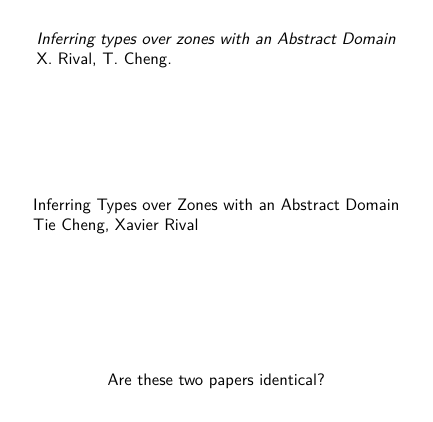
\begin{tikzpicture}[scale=0.6,every node/.style={scale=0.6}]
        \node[align=left] (l) {\emph{Inferring types over zones with an Abstract Domain} \\
     X. Rival, T. Cheng.};

 \node[align=left] at (0,-3.5) (r) {Inferring Types over Zones with an Abstract Domain \\
 Tie Cheng, Xavier Rival};

  \node at (0, -7) {Are these two papers identical?};


    \end{tikzpicture}


}

\column{0.33}
\block{Similarity clustering}{
    Author names are ambiguous, because researchers
    may share the same name or change names. To reduce this
    ambiguity, we cluster papers involving similar author names
    to identify which were written by the same person.
    
    We use a \textbf{semi-supervised} approach based on a binary
    classifier trained to predict whether similar names in two
    papers refer to the same person. This defines a graph where
    connected components correspond to researchers.


    \vspace{1cm}
    \hspace{-2.4cm}
    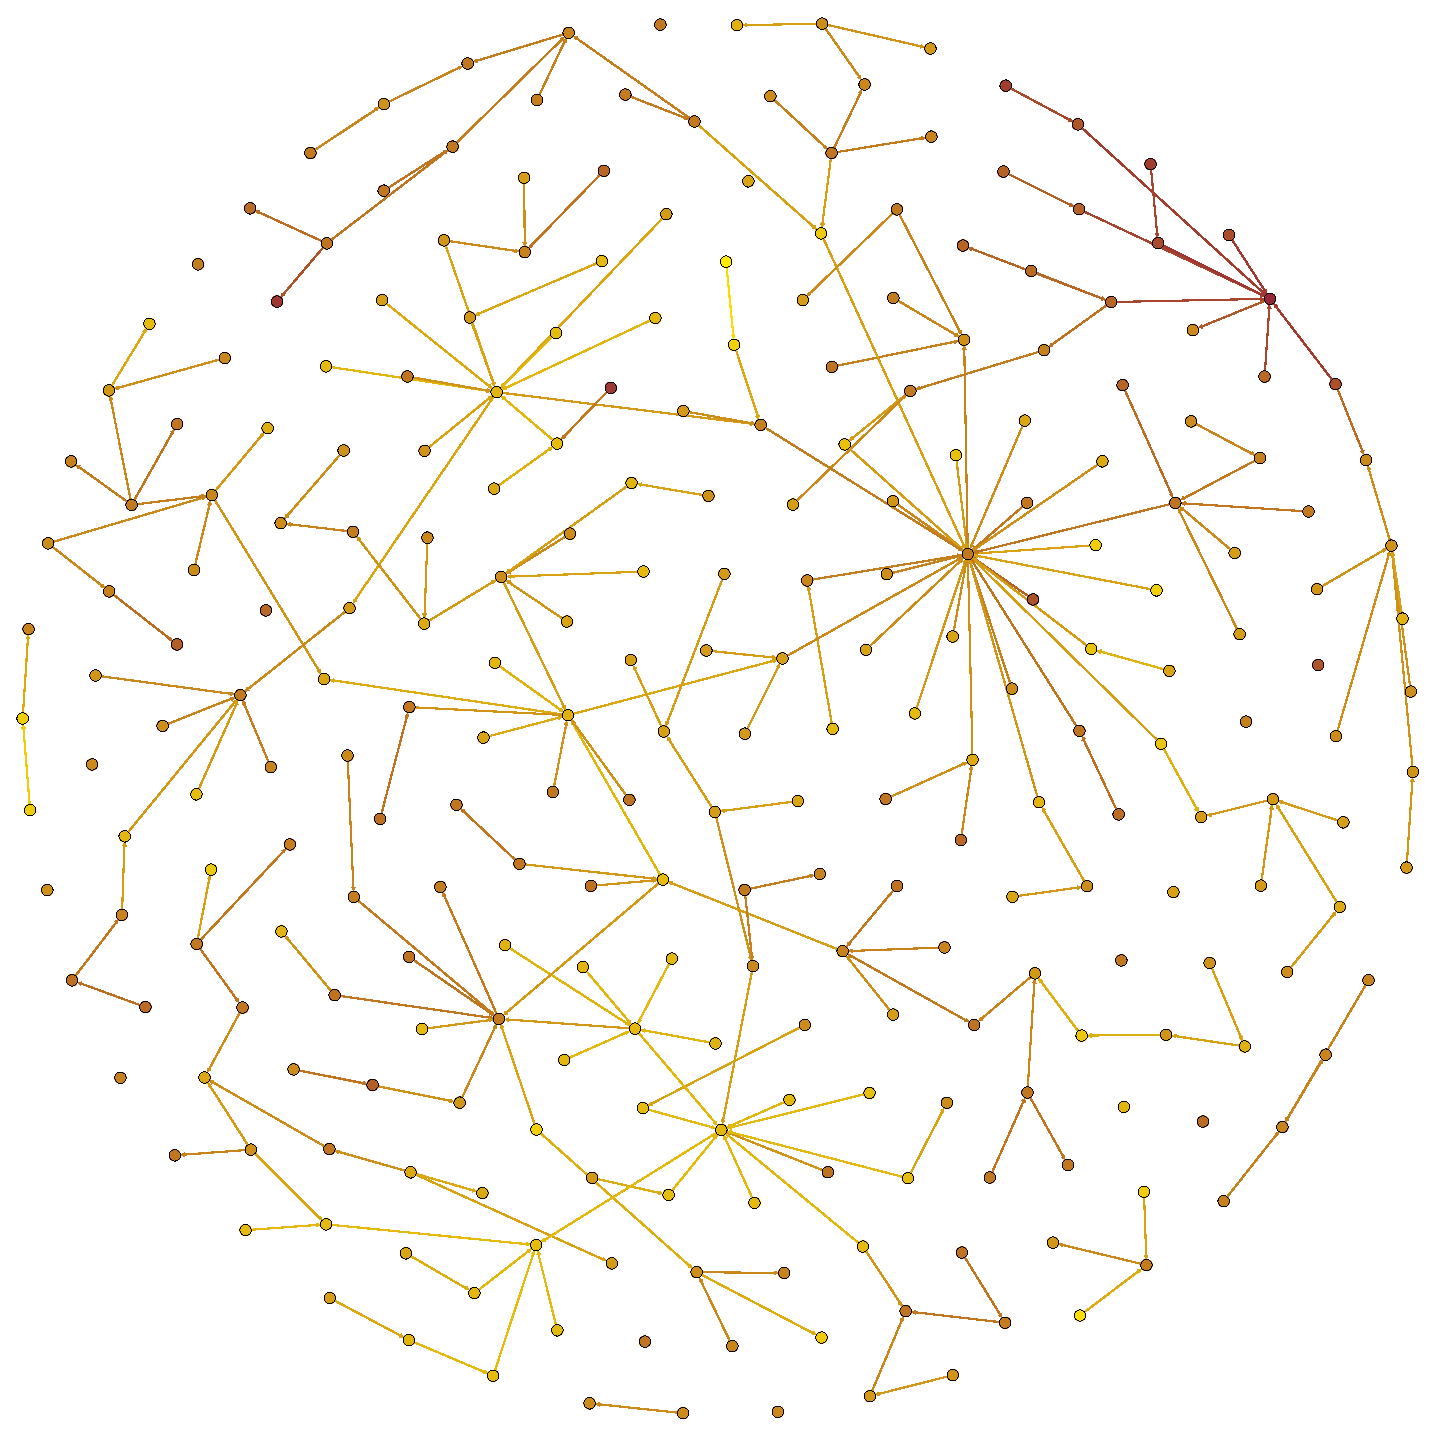
\includegraphics[scale=0.8]{figures/clustering.eps}

    {\small Spanning tree created by the classifier for \emph{Zhen Zhang}}

    Our classifier is trained on a set of 2035 manually annotated
    papers where authors have been identified. We randomly
    generate positive and negative training pairs of example
    papers to train a Support Vector Machine with linear kernel.
    
    \vspace{1cm}
    \begin{tikzpicture}[scale=0.6,every node/.style={scale=0.6}]
        \node[align=left] (l) {\emph{\framebox[1.05\width]{An Abstract Domain} Combinator for Separately} \\
            \emph{Conjoining Memory Abstractions}\\
     Antoine Toubhans, Bor-Yuh Evan Changi, \textbf{Xavier Rival.} \\
 \framebox[1.05\width]{Lecture Notes in Computer Science}, 2014};

 \node[align=left] at (-0.8,-6) (r) {Inferring Types over Zones with \emph{\framebox[1.05\width]{an Abstract Domain}} \\
      Tie Cheng, \textbf{Xavier Rival} \\
  \framebox[1.05\width]{Lecture Notes in Computer Science}, 2012};

  \draw (-3,2.5) .. controls (11,5) and (16,0) .. (10,-4);
  \draw (-11.7,-2.5) edge[bend right] (-11.7,-6.7);

  \node at (0, -10) {Are these two \textbf{Xavier Rival} the same person?};


    \end{tikzpicture}

    Our features use unigram language models to model the similarity
    between metadata fields, and name similarity heursitics to compare
    authors.
}

\column{0.33}
\block{Relevance estimation}{
    Once the papers are clustered, we assess their relevance for
    particular researchers. We learn a topic model for each department 
    and use it to score each paper. The score is averaged over each
    connected component in the graph and attributed to the target
    researcher if the overall score for the component is positive.

    \vspace{-1.8cm}
}

\block{Results}{
    We test our system to gather the publications of 642 researchers
    from the University of Cambridge. This demonstrates that
    many publications could be made freely available but cannot be found
    in the repositories we cover.
    \vspace{0.5cm}

    \hspace{-2cm}
    \begin{tabular}{r c c c}
           & Available & Unavailable & Overall \\
        \hline
        OA & 1952 & 0 & 1952 \\
        Permissive & 2499 & \textbf{5654} & 8153 \\
        Not permissive & 1176 & 82 & 1258 \\
        Unknown & 2080 & 2769 & 4849 \\
        \hline
        Total & 6613 & 9599 & 16212 \\
        \hline
    \end{tabular}
    \vspace{0.3cm}

    The list of papers annotated with their status can be browsed online:
    \vspace{0.5cm}

    \hspace{-2cm}
    
\includegraphics{figures/rendered_papers.eps}

    \vspace{-2cm}
}
\block{References}{
    \nocite{weiler2011authormagic}
    \renewcommand\refname{}
    \vspace{-2cm}
    {\small
    \bibliographystyle{plain}
    \bibliography{references}
}
}





\end{columns}


\end{document}
